\chapter{Analisi dei requisiti}
\label{ch:analisi}

Prima di procedere nella progettazione è fondamentale analizzare il problema per poi costruire un modello che soddisfi i requisiti trovati. Per tale scopo prima vengono prima riportati i risultati del lavoro di Michele Spina, tra cui parte delle interfacce grafiche sviluppate, dopodiché si procede con la modellazione più approfondita e precisa.

\section{Origine della funzionalità}

La necessità di trovare uno spazio di interazione sociale, per lo scambio di informazioni relative alle scosse più recenti, è risultata da un lavoro di interviste del tirocinante Daniele Proietti. In seguito il tirocinante Michele Spina ha preso in carico i risultati per progettare più nel dettaglio la funzionalità, ponendo attenzione sulle interfacce utente per sistema operativo Android. L'attuale sistema di segnalazioni presente in SeismoCloud differisce dalla necessità scoperta in base ai soggetti di questi due sistemi: nel primo caso sono i sismometri che inviano le rilevazioni sismiche, nel secondo caso sono gli utenti che interagiscono tra di loro.

\paragraph{Perché le chat?} La scelta di utilizzare un approccio basato su chat deriva dell'estrema diffusione di sistemi di messaggistica, per cui l'utente non dovrebbe avere difficoltà a utilizzare questo nuovo sistema. C'è però una differenza sostanziale di fondo, poiché il nuovo sistema è focalizzato sul dominio di SeismoCloud, cioè i terremoti, mentre un sistema generale di messaggistica non ha uno scopo preciso. Questo fatto è importante per capire le decisioni prese nella modellazione delle funzionalità.

\paragraph{Elenco delle chat} L'utente può interagire con altri in delle chat pubbliche, dei luoghi in cui si possono inviare e ricevere dei messaggi di varia tipologia. La figura \ref{fig:android_menu} mostra la schermata principale da cui l'utente può selezionare la singola chat. L'elenco è ordinato dalla chat aggiornata più di recente. Nell'interfaccia si possono notare dettagli importanti tra cui: il nome della chat, legato al luogo nel quale sono state sentire le scosse, un'anteprima dell'ultimo messaggio, un contatore dei messaggi non letti e la data, o l'ora, dell'ultimo aggiornamento.

Si sottolinea che le chat sono pubbliche e accessibili sia in scrittura che in lettura per tutti gli utenti, in modo indifferente dalla loro posizione geografica. Il motivo è che un utente lontano dal sisma potrebbe voler chiedere informazioni su quanto accaduto.

\paragraph{I messaggi} Una volta selezionata la chat, l'utente, oltre a inviare un messaggio, può scorrere la cronologia dei messaggi inviati, come mostrato nella figura \ref{fig:android_chat}. Per ogni messaggio è indicato il nome del mittente, la località di invio del messaggio e l'ora di invio. Ci sono tre tipologie di messaggi previsti:

\begin{itemize}
\item Messaggi testuali, che contengono soltanto testo;
\item Messaggi fotografici, che consistono in una singola foto;
\item Messaggi \textit{slider}, che consistono in un valore numerico, rappresentato come slider, cioè una barra orizzontale composta da passi, ognuno dei quali rappresenta un valore, accompagnato da una formula testuale esplicativa che è prefissata.
\end{itemize}

Tra le tre tipologie quello unico e particolare, non presente in altri sistemi di messaggistica, è lo slider. Il valore viene fatto corrispondere alla scala macrosismica Mercalli-Cancani-Sieberg (MCS-1930) \cite{mcs}, con i primi tre valori accorpati perché rappresentano scosse talmente leggere da essere difficilmente rilevabili da un essere umano. La figura \ref{fig:android_slider} è un esempio di un messaggio slider con un valore corrispondente al quarto grado VI della scala.

Riguardo l'invio di un messaggio, la barra inferiore contiene i pulsanti necessari per inviare un messaggio per ogni tipo. Un messaggio può essere inviato opzionalmente con la posizione geografica approssimativa.

\paragraph{Creazione di una chat} Nella barra in alto della schermata principale è possibile premere un pulsante per avviare la creazione di una chat. Una chat è vincolata alla posiziona geografica dell'utente che la crea, per cui l'utente è obbligato a condividere la posizione geografica. La creazione di una chat non è libera, è il sistema a decidere se creare la chat basandosi sulla posizione e sulla data e ora della richiesta. Il nome delle chat è generato in automatico dal sistema, e appena viene creata diventa visibile nell'elenco solo dopo l'invio di un primo messaggio.

\begin{figure}[p]
\centering

% Trucco con minipage per posizionare due figure una accanto all'altra con le loro rispettive didascalie. Attenzione agli spazzi e ai ritorni a capo, non ci devono essere in mezzo altrimenti non funziona!
\begin{minipage}{0.45\linewidth}
\centering
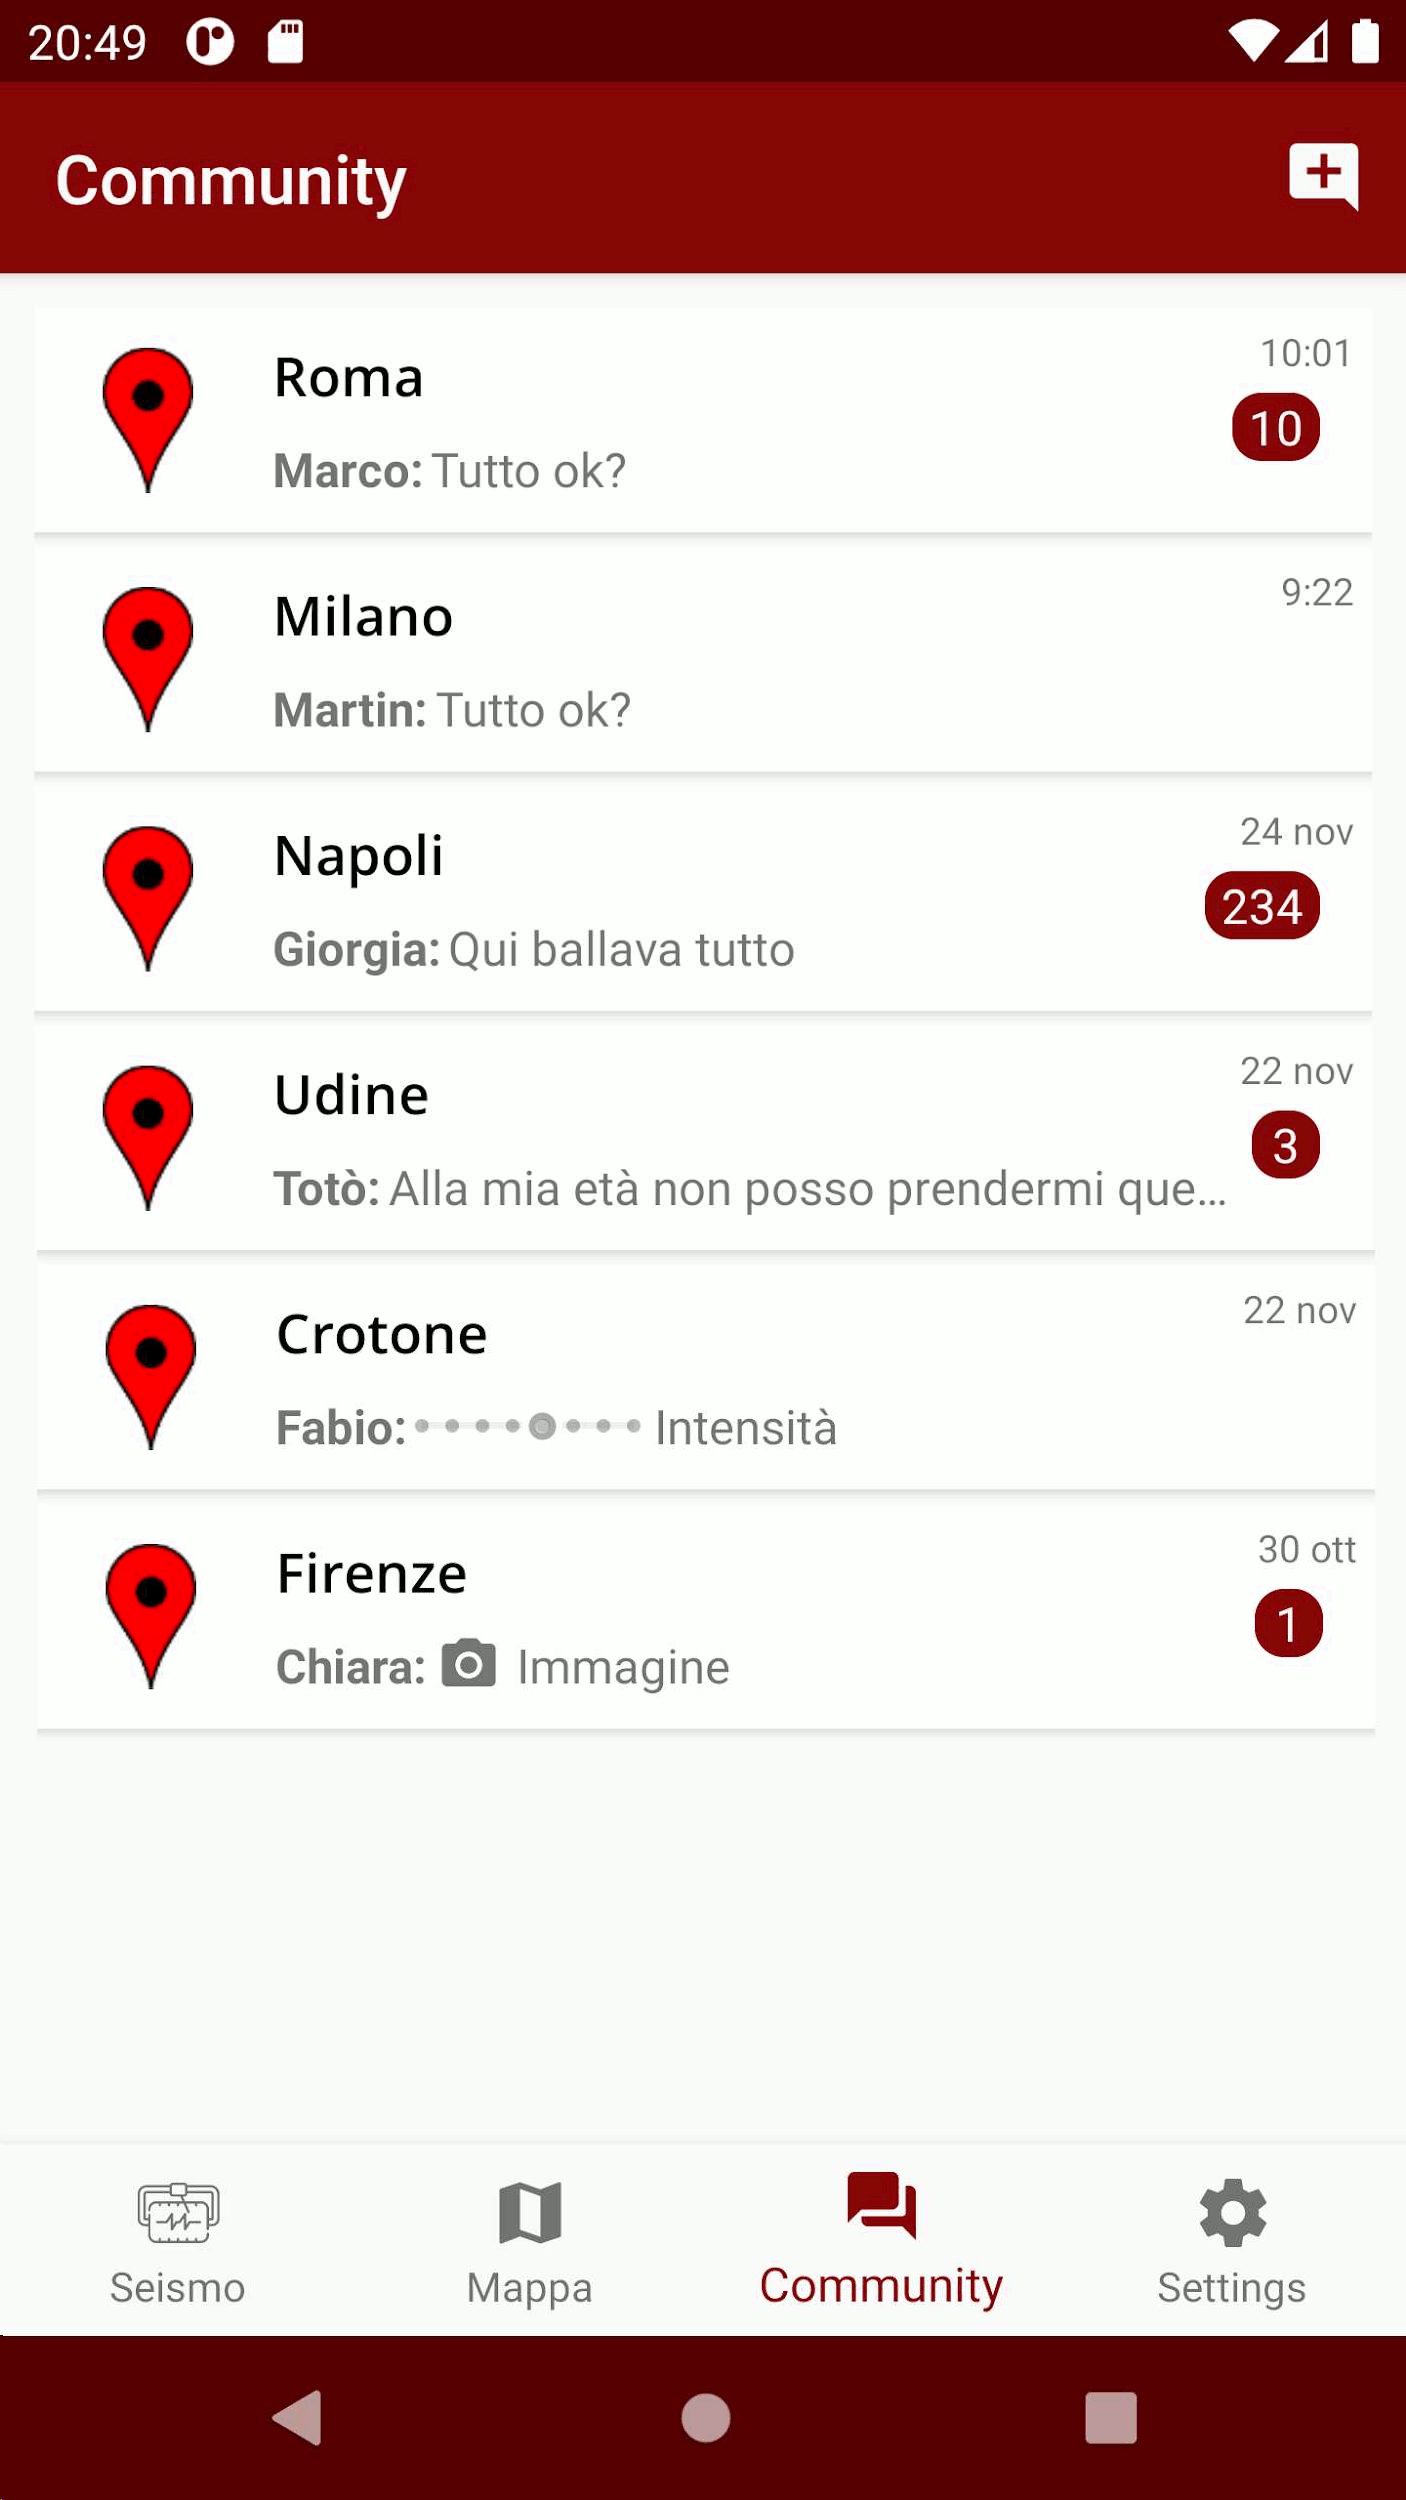
\includegraphics[width=0.85\linewidth]{assets/02/menu.png}
\caption{Schermata con l'elenco delle chat.}
\label{fig:android_menu}
\end{minipage}\hfill
\begin{minipage}{0.45\linewidth}
\centering
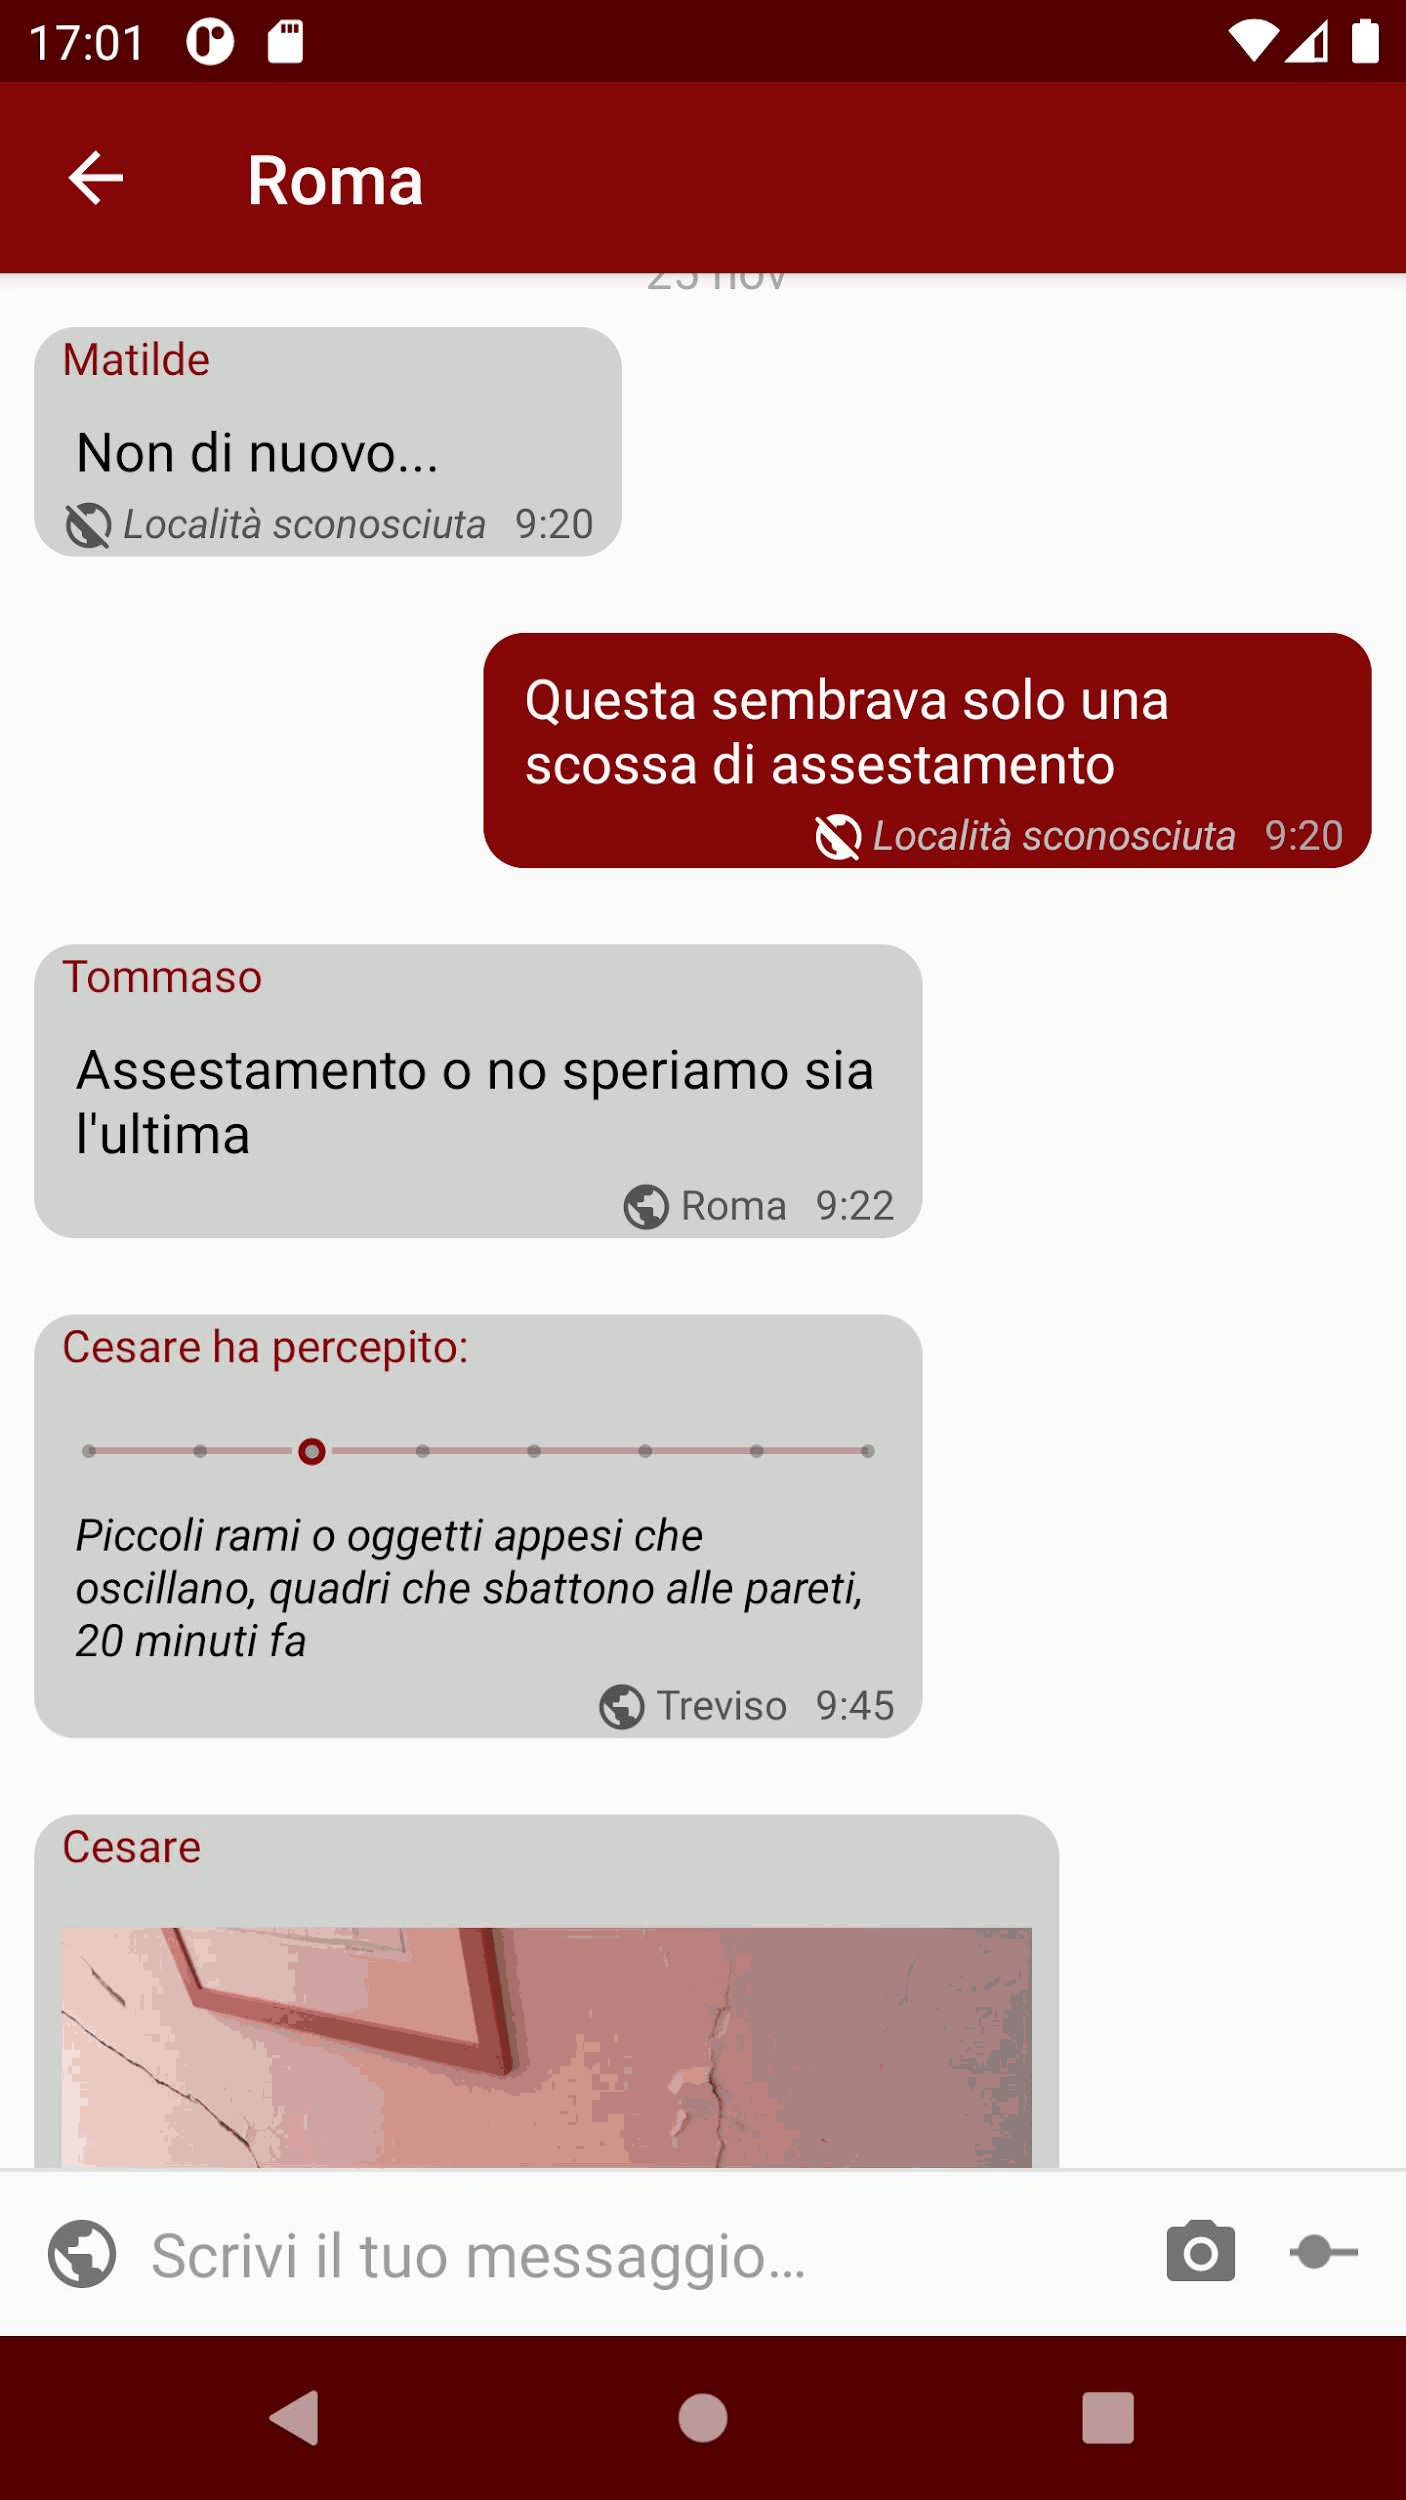
\includegraphics[width=0.85\linewidth]{assets/02/chat.png}
\caption{Schermata visualizzazione chat.}
\label{fig:android_chat}
\end{minipage}

\end{figure}

\begin{figure}[p]
\centering

\begin{minipage}{0.45\linewidth}
\centering
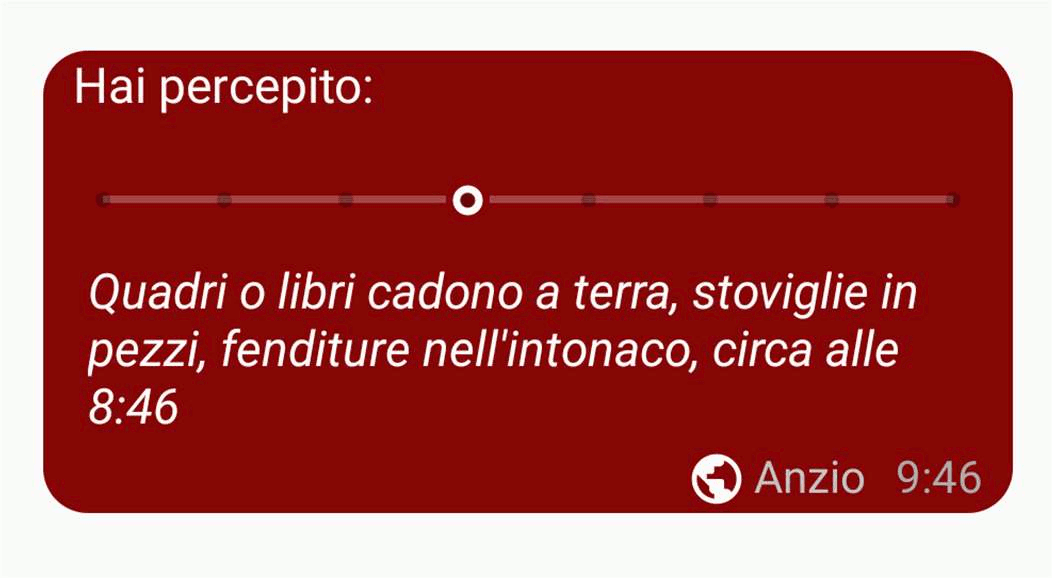
\includegraphics[width=0.85\linewidth]{assets/02/slider.png}
\caption{Dettaglio di un messaggio di tipo slider.}
\label{fig:android_slider}
\end{minipage}\hfill
\begin{minipage}{0.45\linewidth}
\centering
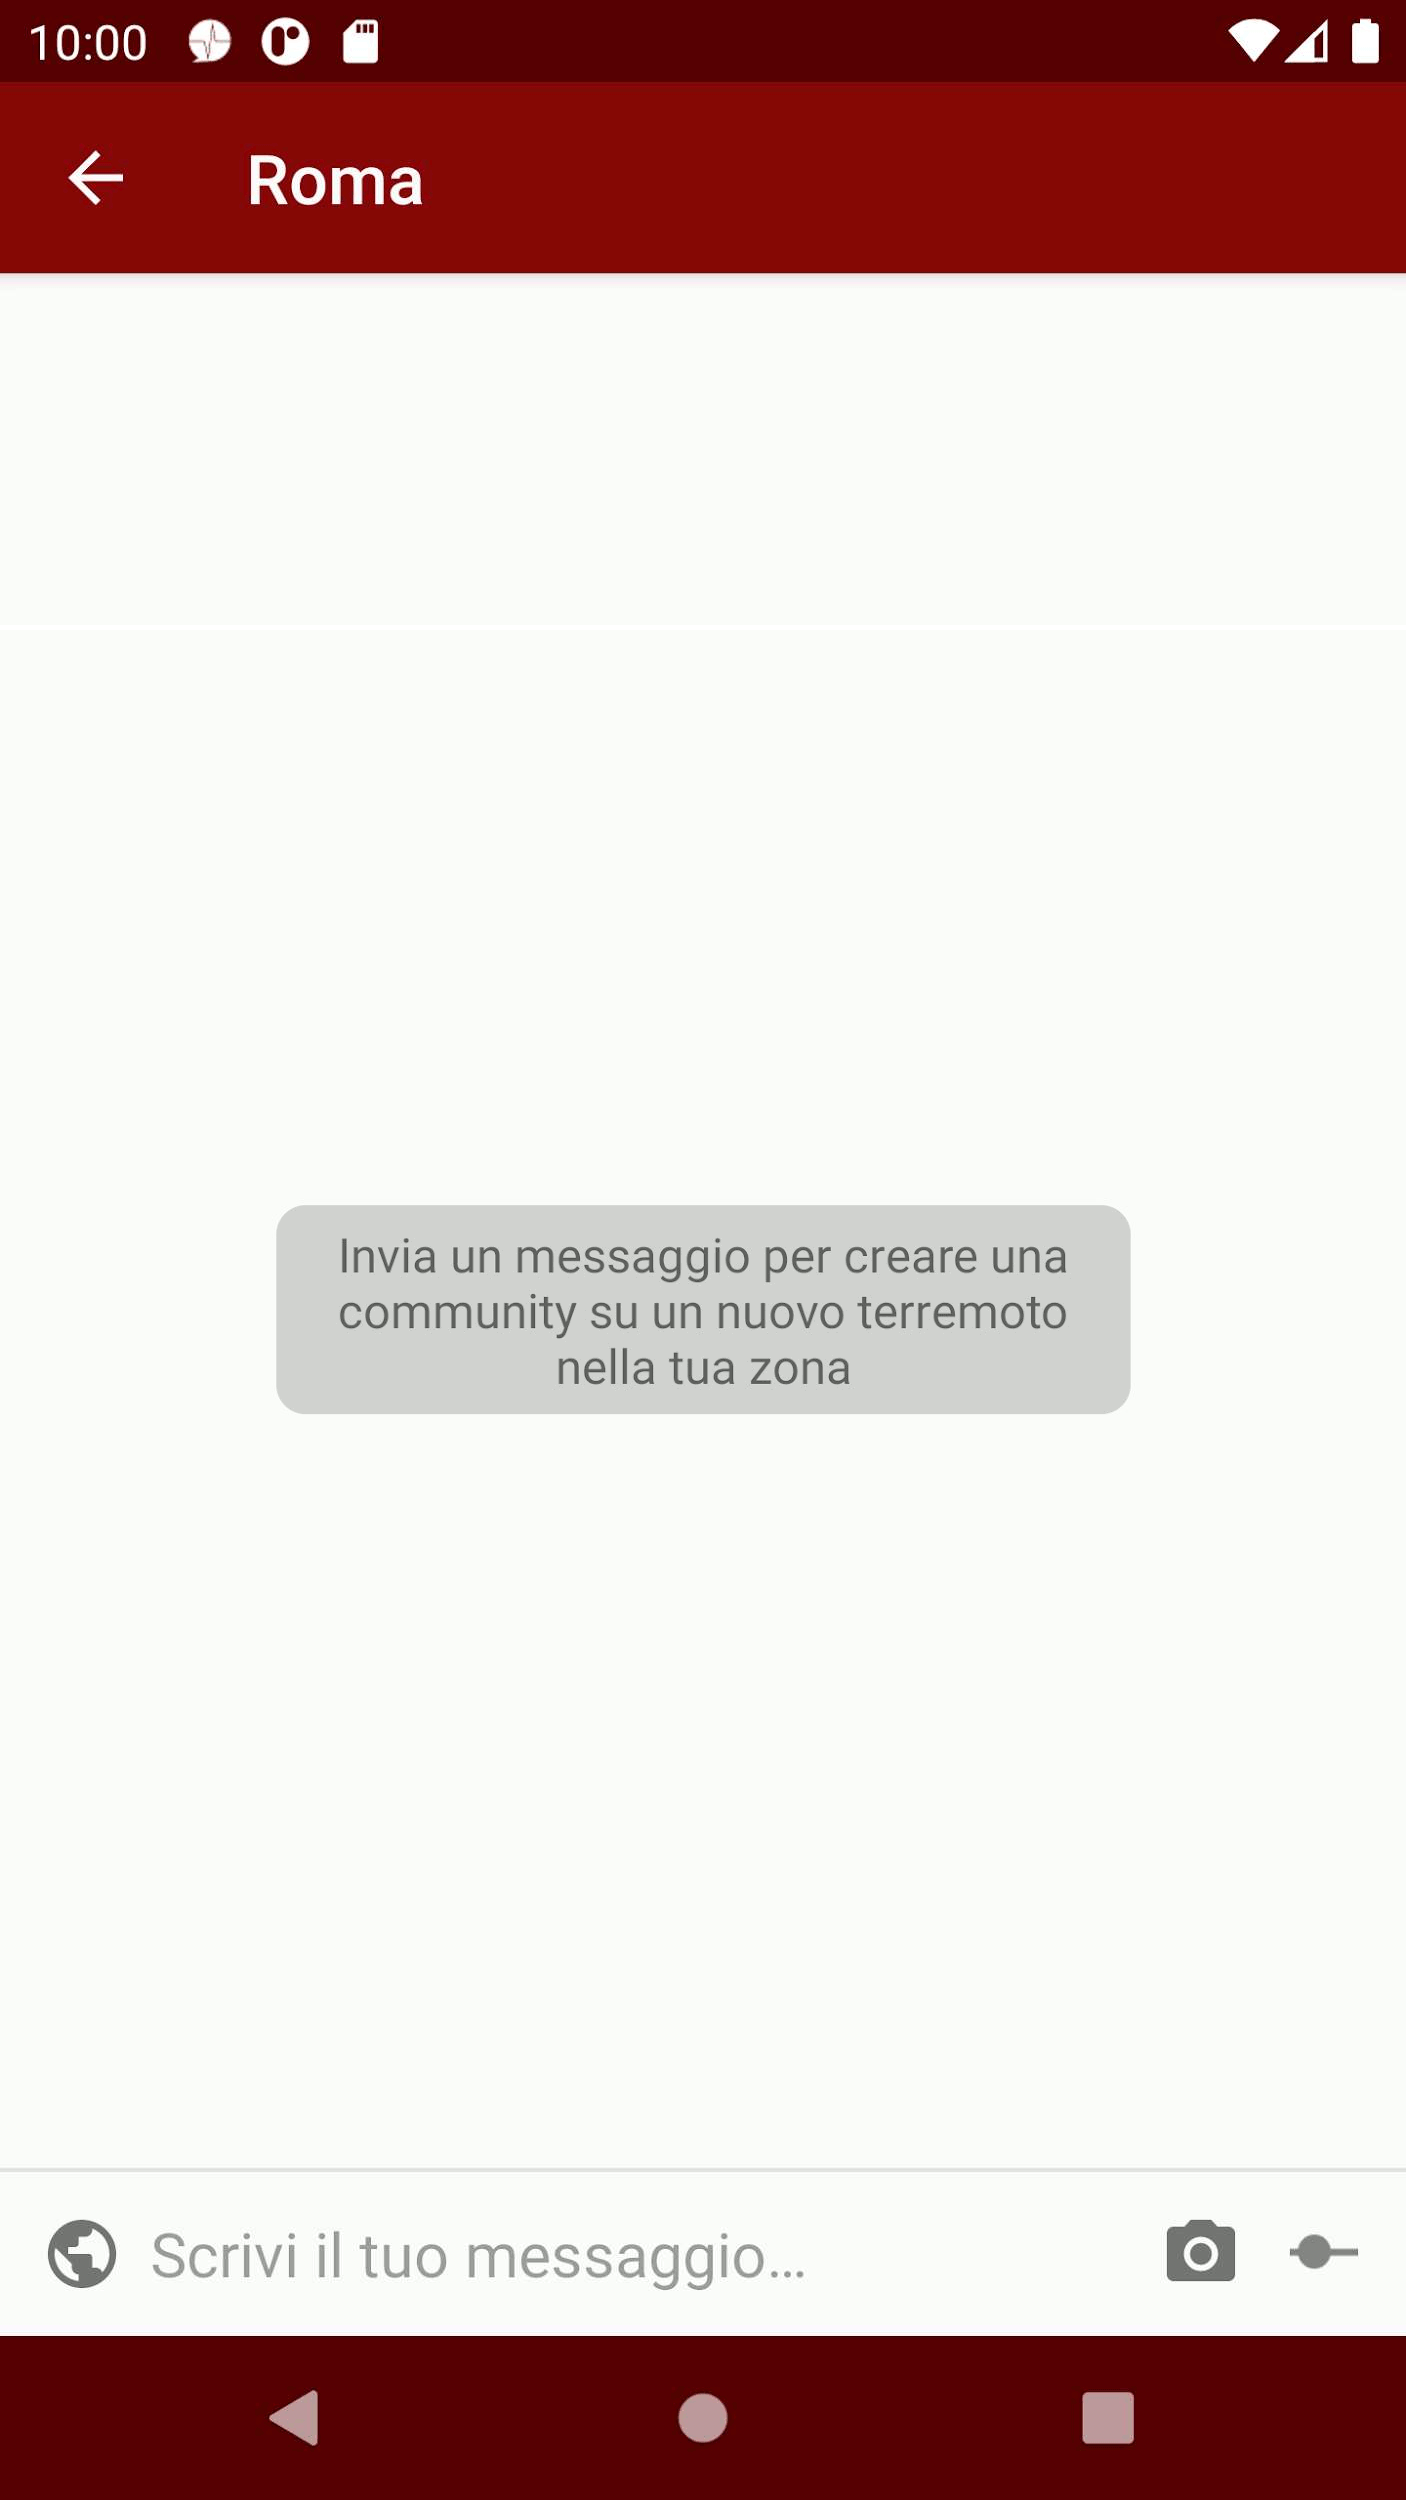
\includegraphics[width=0.85\linewidth]{assets/02/nuova_chat.png}
\caption{Schermata creazione di una chat.}
\label{fig:android_creazione}
\end{minipage}

\end{figure}

\section{Modellazione}

Il lavoro di Michele Spina lascia molte questioni aperte sulla funzionalità che vanno affrontate nella modellazione, progettazione e implementazione di una versione minimale ma effettivamente funzionante.

\paragraph{Dimensioni del modello} Una considerazione generale è stata fatta è sulle dimensioni del modello e quindi del numero di funzionalità da sviluppare. Si è preferito modellare e sviluppare un sistema piccolo ma completo, che soddisfi i principali requisiti, rispetto a uno complesso ma ricco di dettagli e funzioni. La ragione è quella di ottenere feedback da parte degli utenti in modo da estendere passo dopo passo il sistema.

\paragraph{Chat} Le chat sono degli spazi pubblici che contengono messaggi e che gli utenti possono accedere ed eventualmente interagire. La figura \ref{fig:chat_ciclo} mostra il ciclo di vita di una chat: nel momento della sua creazione non è \textit{verificata}, cioè non è stata associata con alcun terremoto; se, entro un termine di tempo specificato, viene effettuata questa associazione, passa nello stato di verificata, altrimenti viene chiusa. Quando una chat è chiusa diventa nascosta agli utenti e non è possibile inviare dei messaggi.

Un fatto importante è che nell'elenco delle chat vengono mostrate solo quelle aperte e solo quelle aggiornate di recente. Significa che l'utente non può scorrere la cronologia completa delle chat. Questa scelta insieme all'associazione con un terremoto derivano dall'obiettivo di tale funzionalità: permette l'interazione nel contesto delle scosse sismiche, scostandosi da un sistema di messaggistica generico.

\begin{figure}[ht!]
\centering
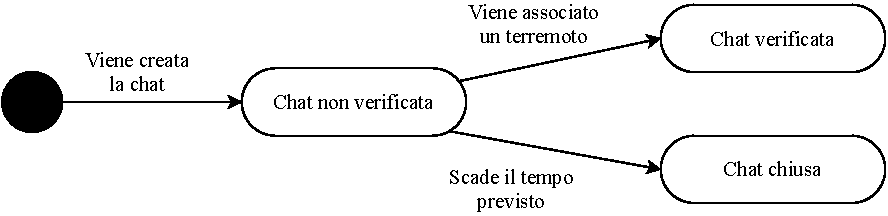
\includegraphics[width=\textwidth]{assets/02/chat_ciclo.pdf}
\caption{Ciclo di vita di una chat.}
\label{fig:chat_ciclo}
\end{figure}

\paragraph{Creazione di una chat} Viene definita una semplice regola per determinare quando una chat deve essere creata o meno: nel momento in cui l'utente richiede la creazione, il sistema analizza tutte le chat create in un arco specifico di tempo prima della richiesta (di solito qualche ora, visto che i terremoti non sono molto frequenti e che più scosse sismiche di un luogo possono essere accorpati in un unico terremoto), quindi per ognuna controlla che la distanza geografica rientri in un'area con centro le coordinate fornite nella richiesta (motivo per cui è obbligatorio che l'utente condivida la posizione) e un raggio specificato a livello di sistema. Se una chat esistente ha riscontro, viene rifiutata la richiesta e indirizzato l'utente sul quella che ha fatto riscontro. La regola pensata è primitiva, ma facilmente estendibile per migliorare la scelta di creazione.

\paragraph{Il ruolo della posizione geografica} Per una chat vengono salvate soltanto le coordinate geografica dell'utente che la crea. Da tali coordinate viene inferito il nome della chat, ponendo attenzione sui capoluoghi di provincia e sulla regione. L'associazione con un terremoto avviene confrontando i dati ufficiali provenienti da INGV \cite{ingv-data} con quelli della chat. Tale associazione non è precisa, è stato comunque deciso per il momento di non complicare ulteriormente il modello, per esempio considerando più coordinate geografiche.

La generazione del nome della chat viene effettuato tramite Nominatim \cite{nominatim}, il sistema fornito da OpenStreetMap per effettuare la geolocalizzazione partendo dalle coordinate geografiche o da un nome (come un indirizzo, una città o una regione).

\paragraph{Messaggi} L'utente può inviare un messaggio in una chat che non è stata chiusa. I tipi di messaggi sono quelli descritti nella sezione precedente. All'interno di una chat un utente può scorrere la cronologia completa dei messaggi. Il sistema rifiuterà messaggi testuali o fotografici che superano i limiti di dimensioni imposto a livello globale.

\paragraph{Username} L'utente per poter inviare un messaggio deve impostare un nome utente non univoco nel sistema. Gli utenti possono riconoscere altri utenti tramite questi nomi, ma non è possibile identificarli in modo univoco poiché i nomi utenti possono essere cambiati.

\paragraph{Sottoscrizioni} L'utente può iscriversi a una chat per ricevere le notifiche dei messaggi inviati. L'iscrizione è automatica nel momento in cui l'utente crea una chat. C'è possibilità di rimuovere un'iscrizione.

\paragraph{Il client} Il modello appena descritto, pur se minimale, si concentra principalmente sui comportamenti e caratteristiche lato server. Dall'altra parte, nel lato client, si aprono molte possibilità non esplorate in questo modello. In alcuni casi l'intervento del server aiuta nell'implementazione di funzionalità aggiuntive lato client, un esempio è l'anteprima dei messaggi che è prevista, mentre il contatore dei messaggi non letti non è previsto per il momento.
